\documentclass[12pt]{article}

\usepackage{amssymb,amsmath,amsthm} % Include AMS Math symbols
\usepackage{graphicx}               % Allows for importation of figures 

\title{ Lab 1 }
\author{ Jacob Hurst }
\date{\today}   % Activate to display a given date or no date


\begin{document}

% Display title
\maketitle
\clearpage

\subsection{Equations}
It has very powerful support for equations such
as these:
\begin{equation}
f(x) = e^{1/2 - \sin(5 \pi    x)}, \label{eq:1} 
\end{equation}
\begin{equation}
p(x) = 1+x+x^2. \label{eq:2} 
\end{equation}

\subsection{Referencing}
\LaTeX also supports a very convenient labeling and referencing system
through the command \texttt{\\label} and \texttt{\\ref}.  Above, equation
(\ref{eq:2}) is a polynomial and the function described by equation
(\ref{eq:1}) is plotted in Figure \ref{fig:1}. 

{\bf Note} that you may have to compile the document two times to get
all the cross-referencing between labels and suto work correctly.

\subsection{Figures}
Figures are also easy to incorporate. It is often best to use a figure
format that is based on vector graphics, e.g. Encapsulated PostScript
(eps). PNG is another good format.  An example is given in Figure \ref{fig:1}. 

\begin{figure}[htb]
\begin{center}
   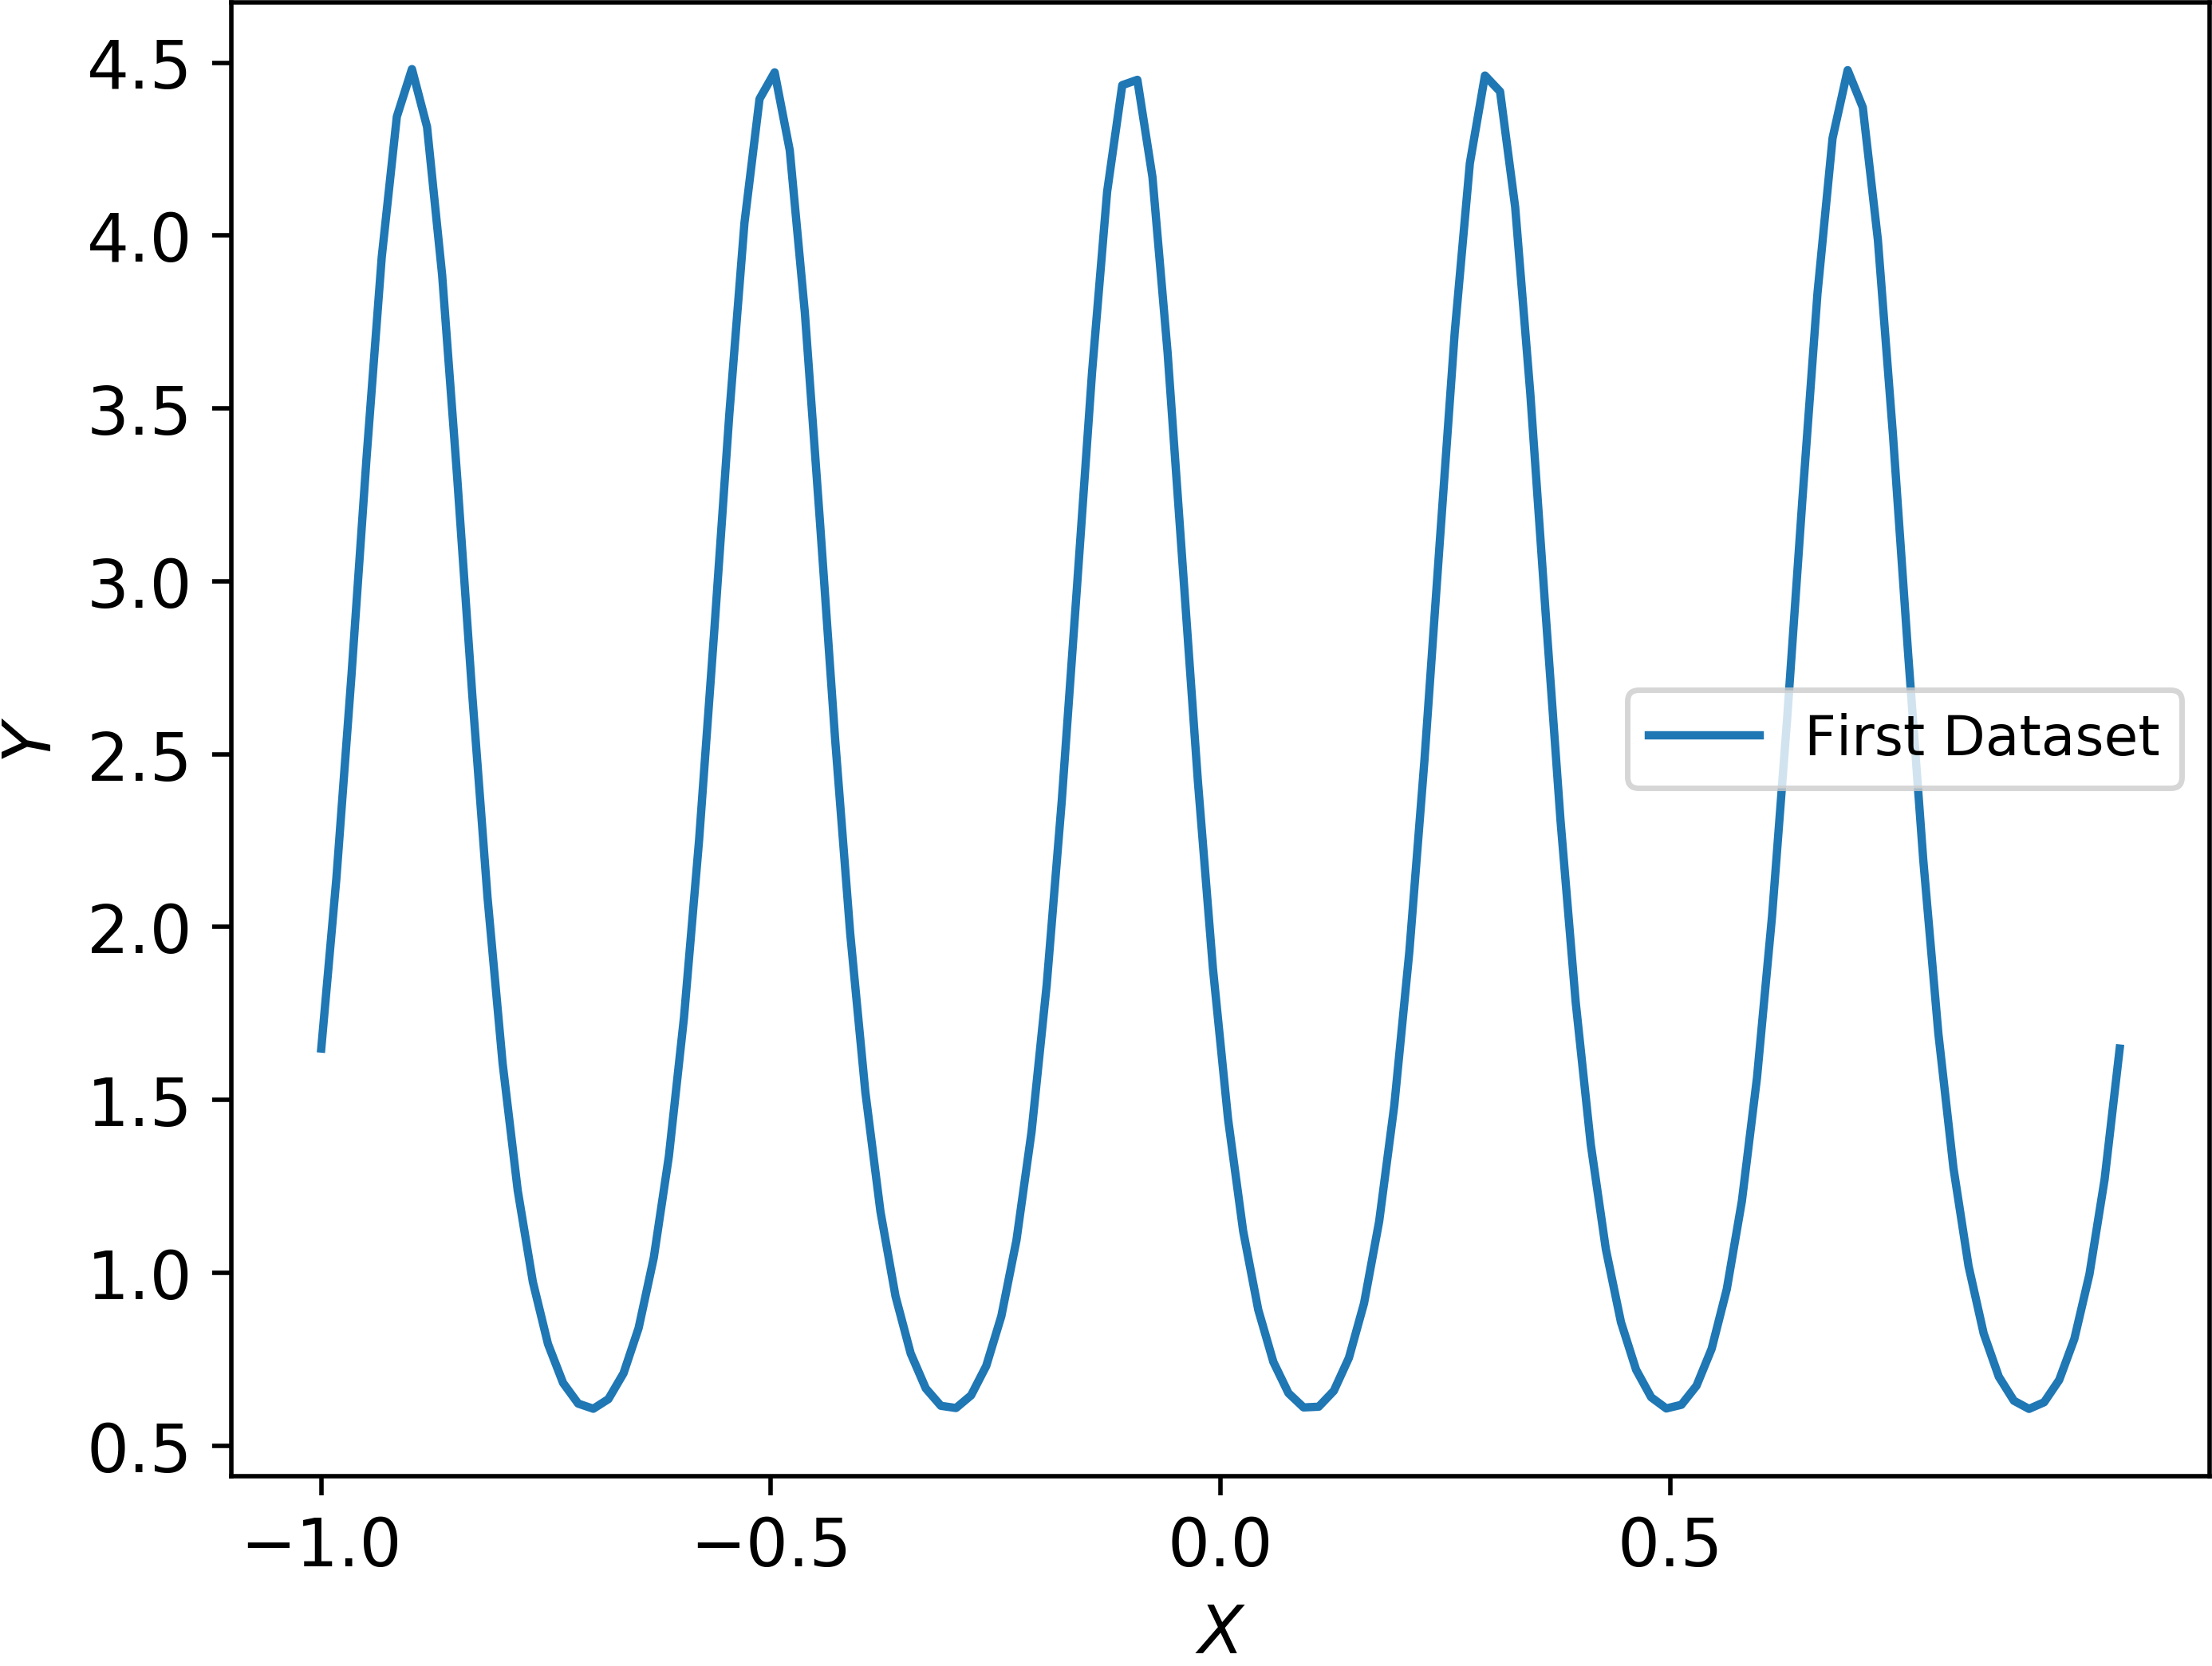
\includegraphics[width=0.32\textwidth]{lab1.png}
   \caption{This figure displays the function $f(x) = e^{1/2 - \sin(5 \pi x)}$.} 
   \label{fig:1}
\end{center}
\end{figure}

\subsection{Tables}
Tables are often useful to display data more compactly than figures.

\begin{table}[h]
\begin{centering}
  \begin{tabular}{| l | c |}
   \hline 
   Breakfast & Spam \\
Lunch & Sausage \\
Dinner & Potatoes \\
  
   \hline
  \end{tabular}
  \caption{A table of delicious meals. \label{tab:1}}
  \end{centering}
\end{table}

\begin{table}[h]
\begin{centering}
  \begin{tabular}{| l | c |}
   \hline 
   1.25000e+00  &  -2.50000e-01 \\
1.02500e+00  &  -2.50000e-02 \\
1.00030e+00  &  -3.04878e-04 \\
1.00000e+00  &  -4.64611e-08 \\
1.00000e+00  &  -1.11022e-15 \\
1.00000e+00  &  0.00000e+00 \\
1.00000e+00  &  0.00000e+00 \\
1.00000e+00  &  0.00000e+00 \\
1.00000e+00  &  0.00000e+00 \\
1.00000e+00  &  0.00000e+00 \\
  
   \hline
  \end{tabular}
  \caption{A table Newton's Method Approximations on (\ref{eq:1}) \label{tab:1}}
  \end{centering}
\end{table}

%\bibliographystyle{plain}
%\bibliography{bibfile}

\end{document}  
